\subsection{Further Mixed Dice-Bce-NQM Losses}
\label{experiments:02.2:FurtherDice-Bce-NQMLosses}
%%%% Intro %%%% 
After and before we had our first successes with the DiceBceNQM loss (\autoref{experiments:02.1:diceBce+NQM}), in the sense that we were able to develop a loss that was no worse than the DiceBCE alone, we tried several other implementations to incorporate the NQM into the DiceBCE loss. However, they were all worse than the DiceBceNQM, or at least no better. However, since the DiceBceNQM was the simplest of the equally good losses, we decided, in the spirit of Occam's razor, to start the robustness experiments (\autoref{experiments:03.0:Intro}) with the DiceBceNQM. The more promising of these were tested again in \autoref{experiments:03.1.x:FurtherNQMLosses}, but showed no improvement over the DiceBceNQM in the experiments here without robustness testing, and were judged here to be more computationally expensive or were developed later and are therefore not yet available. These losses are presented in \autoref{experiments:03.1.x:FurtherNQMLosses} and are omitted here to avoid duplication, even though they are clearly better. For the sake of completeness, we list here the loss functions that are worth mentioning, even if they did not make it to the next round.

For the case of the additive DiceBceNQM (\autoref{experiments:02.1:diceBce+NQM}), we also tested whether taking only Dice+NQM or only Bce+NQM had a positive effect, but as suspected, this was not the case.


%%%% Offen / TODO %%%%
\iffalse
... hier stimmte irgendwas nicht ...
... diceBceMasks (Bce with no reduction) was used and the nqm was put in as weight, before the mean was build ... therefore the nqm was calculated pixelwise ... but did not work
\begin{align}
    \mathrm{DiceBceMaskNQM}     &= \mathrm{DiceLoss} + \mathrm{mean} (NQM_mask \cdot \mathrm{BCE})\\
    \mathrm{BCE}(x,y)           &=  -[y_n \cdot \log x_n + (1-y_n) \cdot \log (1-x_n)]\\
    \mathrm{DiceLoss}           &= 1 - \frac{2 \cdot {\sum^D(y \cdot f_\theta(x))}}
                                            {\sum^D(f_\theta(x)) + \sum^D(f_\theta(x))}
\end{align}
... diceBce SD
... Bce weighted with NQM


\fi
%%%% Inputs %%%%
\paragraph{NQM Loss on Pretrained Model}
\label{experiments:02.2.1:Only_NQM_Pretrained}
As a first "naive" test to circumvent the problems in \autoref{experiments:01.1:Only_NQM}, before we developed the DiceBceNQM (\autoref{experiments:02.1:diceBce+NQM}), we have taken a pretrained models with the DiceBCE.

\begin{align}
    \ell(y_i, f_\theta(x_i))\ :=
      \begin{cases}
        \mathrm{DiceBCE} & \text{if epoch {\color{red}$\leq n$}}\\
        \mathrm{NQM} & \text{else}\\
      \end{cases}
\end{align}

Regardless of how long the model was pretrained, as soon as the loss was switched to the NQM the loss dropped enormously quickly towards zero, for the same reason, as for the NQM alone. The output looks the same as in \autoref{fig:exp.01.1:DiceBce_vs_NQM_only} (left).

%%% Alternating
Since it is only a little adjustment form there, we also checked, if this can already be prevented if we alternate between the NQM and DiceBCE. So the loss becomes:

\begin{align}
    \ell(y_i, f_\theta(x_i))\ :=
      \begin{cases}
        \mathrm{NQM} & \text{if epoch {\color{red} mod $x=0$}}\\
        \mathrm{DiceBce} & \text{else}\\
      \end{cases}
\end{align}

However, this attempt suffers from the same problem. For comparison, \autoref{fig:exp.02.1:alternating} shows that already after three epochs on the NQM, the output looks as bad as \autoref{experiments:01.1:Only_NQM} and moreover, already in the very first epoch no useful prediction is left anymore So, for larger $x$ this attempt only takes longer but still converges to the same state, while the epochs with the DiceBCE work in the opposite direction.

\begin{figure}[h!]
    \centering
    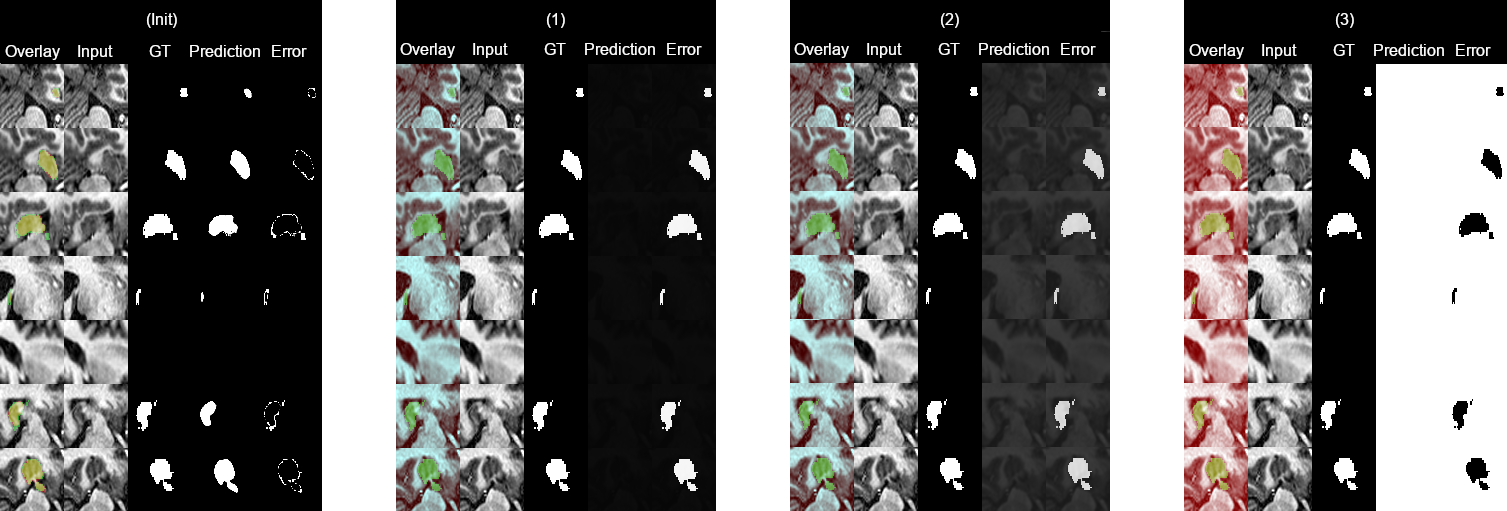
\includegraphics[width=\linewidth]{Graphics/Experiments/4.2.1_Alternating_3epochs_v3.png}
    \caption{Image samples volumes (inputs) with ground truth labels (GT), predictions, and errors. The overlay shows the input image with false positive (red), true positive (yellow), and  false negative (green). From left to right: The initial state, pretrained on DiceBCE (Init), the three very first epochs of training on the NQM.}
    \label{fig:exp.02.1:alternating}
\end{figure}
\paragraph{Multiplicative Dice-Bce-NQM Losses}
\label{experiments:02.2.2:dice+NQM}
To give the NQM more weight in the loss, we also used the NQM as a factor before the DiceBCE. Therefore, we tested the following three implementations of a multiplicative DiceBceNQM loss. However, they all suffered from the same problem as the NQM alone (\autoref{experiments:01.1:Only_NQM}) and the pretrained versions (\autoref{experiments:02.2.1:Only_NQM_Pretrained}). DiceBce*NQM-2 and 3 canceled only the part that has been multiplied with the NQM. Therefore, we tested, with the NQM as defined in \autoref{eq:02.1:Only_NQM}:

\begin{align}
    \text{DiceBce*NQM-1}\ &:=\ {\color{red}\mathrm{NQM}\ \cdot\ }(1 - \mathrm{Dice} + \mathrm{Bce})\\
    \text{DiceBce*NQM-2}\ &:=\ {\color{red}\mathrm{NQM}\ \cdot\ }(1 - \mathrm{Dice}) + \mathrm{Bce}\\
    \text{DiceBce*NQM-3}\ &:=\ 1 - \mathrm{Dice} + {\color{red}\mathrm{NQM}\ \cdot\ }\mathrm{Bce}\\ 
\end{align}